\documentclass[aspectratio=169,11pt]{beamer}

\usepackage{fontspec}
\usepackage{booktabs}
\usepackage{tabularx}
\usepackage{array}
\usepackage{amsmath}
\usepackage{xcolor}
\usepackage{tikz}
\usetikzlibrary{arrows.meta,positioning,fit,calc,shapes.geometric,decorations.pathreplacing}

\setmainfont{Helvetica Neue}
\setsansfont{Helvetica Neue}
\setmonofont{Menlo}

\definecolor{HUSTBlue}{RGB}{0,63,164}
\definecolor{HUSTDeep}{RGB}{7,34,86}
\definecolor{HUSTCyan}{RGB}{0,150,170}
\definecolor{HUSTGreen}{RGB}{38,160,82}
\definecolor{HUSTOrange}{RGB}{226,132,28}
\definecolor{HUSTRed}{RGB}{196,0,0}
\definecolor{HUSTPurple}{RGB}{112,86,205}
\definecolor{HUSTLight}{RGB}{238,244,253}
\definecolor{HUSTLine}{RGB}{150,175,215}
\definecolor{HUSTGray}{RGB}{82,92,110}

\usetheme[progressbar=frametitle,numbering=fraction]{metropolis}
\usefonttheme{professionalfonts}
\setbeamersize{text margin left=0.72cm,text margin right=0.72cm}
\setbeamertemplate{navigation symbols}{}
\metroset{block=fill,titleformat=regular,sectionpage=none}
\setbeamercolor{normal text}{fg=black,bg=white}
\setbeamercolor{progress bar}{fg=HUSTBlue,bg=HUSTLine}
\setbeamercolor{frametitle}{fg=HUSTBlue,bg=white}
\setbeamerfont{frametitle}{series=\bfseries,size=\large}
\setbeamercolor{title}{fg=HUSTBlue}
\setbeamerfont{title}{series=\bfseries,size=\huge}
\setbeamercolor{author in head/foot}{fg=HUSTGray,bg=white}
\setbeamercolor{page number in head/foot}{fg=HUSTBlue,bg=white}
\setbeamercolor{block title}{fg=HUSTBlue,bg=HUSTLight}
\setbeamercolor{block body}{fg=black,bg=HUSTLight!55}
\setbeamercolor{alerted text}{fg=HUSTRed}
\setbeamercolor{itemize item}{fg=HUSTBlue}
\setbeamercolor{itemize subitem}{fg=HUSTCyan}
\setlength{\parskip}{0.05cm}
\setbeamertemplate{itemize/enumerate body begin}{\setlength{\itemsep}{0.16cm}}
\setbeamertemplate{itemize/enumerate subbody begin}{\setlength{\itemsep}{0.08cm}}

\newcommand{\key}[1]{\textcolor{HUSTDeep}{\textbf{#1}}}
\newcommand{\term}[1]{\textcolor{HUSTBlue}{\textbf{#1}}}
\newcommand{\smallnote}[1]{\textcolor{HUSTGray}{\footnotesize #1}}
\newcommand{\tagbox}[2]{%
  \begin{tikzpicture}[baseline=(n.base)]
    \node[rounded corners=2pt, draw=#1, fill=#1!8, inner xsep=4pt, inner ysep=2pt, font=\scriptsize\bfseries, text=#1] (n) {#2};
  \end{tikzpicture}%
}
\newcolumntype{Y}{>{\raggedright\arraybackslash}X}
\newcommand{\topicsectionpage}[2]{%
  \begin{frame}[plain]
    \vspace{1.0cm}
    {\huge\bfseries\textcolor{HUSTBlue}{#1}}\par
    \vspace{0.26cm}
    {\large\textcolor{HUSTGray}{#2}}\par
    \vfill
    \textcolor{HUSTLine}{\rule{0.76\paperwidth}{0.8pt}}
  \end{frame}
}
\newcommand{\breakpage}[2]{%
  \begin{frame}[plain]
    \vspace{1.0cm}
    {\huge\bfseries\textcolor{HUSTBlue}{10-Minute Break}}\par
    \vspace{0.28cm}
    {\Large\textcolor{HUSTGray}{#1}}\par
    \vspace{0.8cm}
    \begin{block}{Before the next session}
      #2
    \end{block}
    \vfill
    \textcolor{HUSTLine}{\rule{0.76\paperwidth}{0.8pt}}
  \end{frame}
}

\title{Large Language Model Inference Systems}
\subtitle{From a User Request to a Production Serving Stack}
\author{Shuhao Zhang \\ School of Computer Science and Technology, HUST}
\date{Three-Hour English Course \\ 2026}

\begin{document}

\begin{frame}[plain]
  \begin{tikzpicture}[remember picture,overlay]
    \fill[HUSTLight!60] ([yshift=-0.18cm]current page.north west) rectangle ([yshift=-0.42cm]current page.north east);
    \draw[HUSTBlue, line width=1.0pt] ([xshift=0.78cm,yshift=-0.90cm]current page.north west) -- ([xshift=5.25cm,yshift=-0.90cm]current page.north west);
    \draw[HUSTCyan, line width=1.0pt] ([xshift=5.35cm,yshift=-0.90cm]current page.north west) -- ([xshift=7.15cm,yshift=-0.90cm]current page.north west);
    \node[anchor=south east, text=HUSTGray, font=\scriptsize, align=right] at ([xshift=-0.78cm,yshift=0.60cm]current page.south east)
      {Three-Hour English Teaching Edition\\2026};
  \end{tikzpicture}

  \vspace{1.42cm}
  {\fontsize{23}{28}\selectfont\bfseries\textcolor{HUSTBlue}{Large Language Model}}\par
  \vspace{0.02cm}
  {\fontsize{23}{28}\selectfont\bfseries\textcolor{HUSTBlue}{Inference Systems}}\par
  \vspace{0.38cm}
  {\Large\textcolor{HUSTDeep}{From one request to a production serving stack}}\par

  \vspace{1.05cm}
  {\large Shuhao Zhang}\par
  \vspace{0.10cm}
  {\normalsize Huazhong University of Science and Technology}\par

  \vspace{0.92cm}
\end{frame}

\begin{frame}{A concrete story: one chatbot question}
  \begin{columns}[T,totalwidth=\textwidth]
    \begin{column}{0.46\textwidth}
      \begin{block}{User sees}
        \begin{itemize}
          \item Type a question.
          \item Wait for the first word.
          \item Watch tokens stream out.
          \item Abandon the task if the service feels slow.
        \end{itemize}
      \end{block}
    \end{column}
    \begin{column}{0.50\textwidth}
      \begin{block}{System does}
        \begin{itemize}
          \item Tokenize and validate the request.
          \item Queue it with other users' requests.
          \item Run prefill to create KV cache.
          \item Run decode for many iterations.
          \item Stream output and recycle memory.
        \end{itemize}
      \end{block}
    \end{column}
  \end{columns}
  \vspace{0.16cm}
  \begin{center}
    \normalsize\term{LLM serving is an online stateful system.}
  \end{center}
\end{frame}

\begin{frame}{Three-hour course roadmap}
  \footnotesize
  \begin{columns}[T,totalwidth=\textwidth]
    \begin{column}{0.32\textwidth}
      \begin{block}{Session 1: model to request}
        \begin{itemize}
          \item Tokens, attention, and Transformer blocks
          \item Autoregressive generation
          \item Prefill, decode, and service metrics
        \end{itemize}
      \end{block}
    \end{column}
    \begin{column}{0.32\textwidth}
      \begin{block}{Session 2: serving engine}
        \begin{itemize}
          \item Request and iteration scheduling
          \item Continuous batching and KV paging
          \item State ownership, reuse, and pressure
        \end{itemize}
      \end{block}
    \end{column}
    \begin{column}{0.32\textwidth}
      \begin{block}{Session 3: systems evidence}
        \begin{itemize}
          \item RAG, MoE, agents, and accelerators
          \item Heterogeneous execution
          \item Benchmarking and open engineering
        \end{itemize}
      \end{block}
    \end{column}
  \end{columns}
  \vspace{0.10cm}
  \begin{block}{Guiding thread}
    Follow the tensor, follow the request, follow the state, and verify the evidence.
  \end{block}
\end{frame}

\begin{frame}{The big picture}
  \centering
  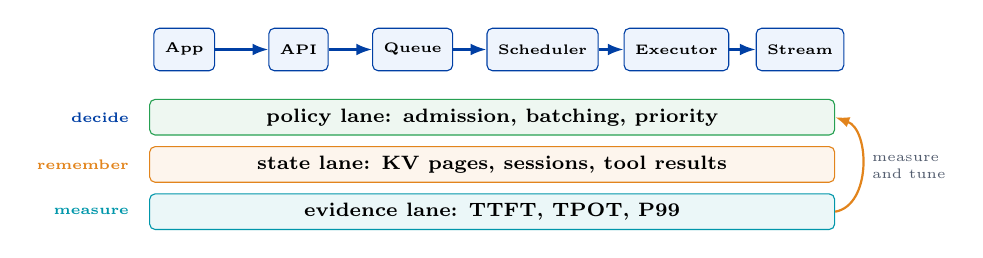
\begin{tikzpicture}[
    x=1cm,y=1cm,
    stage/.style={rounded corners=2pt, draw=HUSTBlue, fill=HUSTLight, minimum height=0.54cm, inner xsep=4pt, align=center, font=\tiny\bfseries},
    lane/.style={rounded corners=2pt, minimum width=8.7cm, minimum height=0.42cm, align=center, font=\scriptsize\bfseries},
    policyplane/.style={lane, draw=HUSTGreen, fill=HUSTGreen!8},
    stateplane/.style={lane, draw=HUSTOrange, fill=HUSTOrange!8},
    metricplane/.style={lane, draw=HUSTCyan, fill=HUSTCyan!8},
    arrow/.style={-{Latex[length=2.0mm]}, thick, draw=HUSTBlue},
    fb/.style={-{Latex[length=1.8mm]}, thick, draw=HUSTOrange}
  ]
    \foreach \x/\name/\lab in {0/app/App,1.45/api/API,2.90/queue/Queue,4.55/sched/Scheduler,6.25/exec/Executor,7.82/stream/Stream} {
      \node[stage] (\name) at (\x,0) {\lab};
    }
    \foreach \a/\b in {app/api,api/queue,queue/sched,sched/exec,exec/stream} {
      \draw[arrow] (\a) -- (\b);
    }
    \node[policyplane] (policy) at (3.91,-0.86) {policy lane: admission, batching, priority};
    \node[stateplane] (state) at (3.91,-1.46) {state lane: KV pages, sessions, tool results};
    \node[metricplane] (metrics) at (3.91,-2.06) {evidence lane: TTFT, TPOT, P99};
    \node[font=\tiny\bfseries, text=HUSTBlue, anchor=east] at (-0.58,-0.86) {decide};
    \node[font=\tiny\bfseries, text=HUSTOrange, anchor=east] at (-0.58,-1.46) {remember};
    \node[font=\tiny\bfseries, text=HUSTCyan, anchor=east] at (-0.58,-2.06) {measure};
    \draw[fb] (metrics.east) to[out=10,in=-20] node[right, font=\tiny, text=HUSTGray, align=left] {measure\\and tune} (policy.east);
  \end{tikzpicture}
  \vspace{0.35cm}
  \begin{itemize}
    \item Many optimizations do not happen inside a single kernel.
    \item They happen at control points: queueing, batching, caching, memory movement, and validation.
  \end{itemize}
\end{frame}

\topicsectionpage{Part I. From Tokens to Autoregressive Inference}{Build the model-side foundation before opening the serving engine}

\begin{frame}{Start with one concrete prompt}
  \begin{block}{Text entered by the user}
    \centering
    \Large ``I love AI.''
  \end{block}
  \begin{enumerate}
    \item The tokenizer splits text into tokens.
    \item Embedding turns each token ID into a vector.
    \item Transformer blocks mix information across positions and channels.
    \item The language-model head scores the next token.
  \end{enumerate}
  \vspace{0.2cm}
  \term{An inference engine serves this computation repeatedly and concurrently.}
\end{frame}

\begin{frame}{Token count is not character count}
  \begin{columns}[T,totalwidth=\textwidth]
    \begin{column}{0.48\textwidth}
      \begin{block}{Teaching example}
        Suppose the tokenizer returns
        \[
          [\texttt{I},\ \texttt{love},\ \texttt{AI},\ \texttt{.}]
        \]
        The sequence length is therefore \(S=4\).
      \end{block}
    \end{column}
    \begin{column}{0.48\textwidth}
      \begin{block}{Do not confuse}
        \begin{itemize}
          \item Text characters
          \item Token IDs
          \item Sequence length \(S\)
          \item Vector width \(d_{\text{model}}\)
        \end{itemize}
      \end{block}
    \end{column}
  \end{columns}
  \vspace{0.25cm}
  If \(d_{\text{model}}=8\), the four token vectors form a \(4\times 8\) matrix.
\end{frame}

\begin{frame}{What question does attention answer?}
  \begin{block}{For every query position}
    Which earlier positions are useful, and how much information should be taken from each one?
  \end{block}
  \begin{itemize}
    \item \(Q\): what the current position is looking for.
    \item \(K\): what each position offers for matching.
    \item \(V\): the information that will actually be mixed.
  \end{itemize}
  \vspace{0.3cm}
  \begin{center}
    \Large\term{Match with \(QK^\top\); mix the \(V\) vectors.}
  \end{center}
\end{frame}

\begin{frame}{Worked attention example: define one row}
  \begin{block}{We compute only the row for token 3: \texttt{AI}}
    Use one head with \(d_{\text{head}}=2\):
    \[
      q_{\text{AI}}=[1,1]
    \]
    \[
      k_{\text{I}}=[1,0],\quad k_{\text{love}}=[0,1],\quad
      k_{\text{AI}}=[1,1],\quad k_{\text{.}}=[0,0].
    \]
  \end{block}
  \begin{itemize}
    \item Four query positions and four key positions create a \(4\times4\) score matrix.
    \item This page follows only its third row; the other rows use the same procedure.
  \end{itemize}
\end{frame}

\begin{frame}{Step 1: compute the four attention scores}
  \[
    \frac{q_{\text{AI}}K^\top}{\sqrt{2}}
    =
    \frac{[1,\ 1,\ 2,\ 0]}{\sqrt{2}}
    \approx
    [0.707,\ 0.707,\ 1.414,\ 0].
  \]
  \begin{enumerate}
    \item Dot product with \texttt{I}: \(1\cdot1+1\cdot0=1\).
    \item Dot product with \texttt{love}: \(1\).
    \item Dot product with \texttt{AI}: \(2\).
    \item Dot product with \texttt{.}: \(0\).
  \end{enumerate}
  \vspace{0.2cm}
  The scale factor \(\sqrt{d_{\text{head}}}\) keeps large dimensions from producing overly sharp scores.
\end{frame}

\begin{frame}{Step 2: the causal mask blocks the future}
  \begin{block}{Token 3 may read positions 1--3, but not position 4}
    \[
      [0.707,\ 0.707,\ 1.414,\ 0]
      \longrightarrow
      [0.707,\ 0.707,\ 1.414,\ -\infty].
    \]
  \end{block}
  \begin{itemize}
    \item The fourth softmax weight becomes zero.
    \item The model cannot use a future token to predict an earlier token.
    \item All known query rows in the same layer can still be computed in parallel.
  \end{itemize}
\end{frame}

\begin{frame}{Step 3: softmax turns scores into weights}
  \[
    \operatorname{softmax}
    ([0.707,\ 0.707,\ 1.414,\ -\infty])
    \approx
    [0.248,\ 0.248,\ 0.503,\ 0].
  \]
  \begin{itemize}
    \item Every weight is non-negative.
    \item The weights sum to approximately one.
    \item These are position-mixing weights for one layer and one head.
  \end{itemize}
  \vspace{0.25cm}
  \key{They are not next-token probabilities over the vocabulary.}
\end{frame}

\begin{frame}{Step 4: attention returns a weighted sum of values}
  Let
  \[
    v_{\text{I}}=[1,0],\quad
    v_{\text{love}}=[0,2],\quad
    v_{\text{AI}}=[2,1].
  \]
  Then
  \[
    o_{\text{AI}}
    =0.248[1,0]+0.248[0,2]+0.503[2,1]
    \approx [1.254,\ 0.999].
  \]
  \begin{block}{Plain-language meaning}
    The representation of \texttt{AI} now contains a weighted mixture of information from visible positions.
  \end{block}
\end{frame}

\begin{frame}{Multi-head attention repeats the same idea}
  \begin{itemize}
    \item Each head has its own \(Q\), \(K\), and \(V\) projections.
    \item Different heads can learn different position relationships.
    \item Head outputs are concatenated and projected back to \(d_{\text{model}}\).
  \end{itemize}
  \vspace{0.25cm}
  \begin{block}{Shape example}
    With \(B=2\), \(S=4\), \(d_{\text{model}}=8\), and two heads:
    \[
      X:2\times4\times8
      \rightarrow
      Q,K,V:2\times2\times4\times4
      \rightarrow
      O:2\times4\times8.
    \]
  \end{block}
\end{frame}

\begin{frame}{A Transformer block preserves the main shape}
  \begin{enumerate}
    \item Normalize the \(B\times S\times d_{\text{model}}\) tensor.
    \item Attention mixes information along the sequence dimension.
    \item Residual addition returns to the main path.
    \item MLP expands and contracts the channel dimension.
    \item A second residual addition completes the block.
  \end{enumerate}
  \vspace{0.28cm}
  \begin{block}{Shape invariant}
    For \(X:2\times4\times8\), the block output is still \(2\times4\times8\).
  \end{block}
\end{frame}

\begin{frame}{The model selects one next token per sequence}
  \begin{block}{After the final Transformer block}
    Take the final position from each sequence, map its \(d_{\text{model}}\)-dimensional vector to \(|V|\) logits, then sample or select one token.
  \end{block}
  \begin{itemize}
    \item Logits are unnormalized vocabulary scores.
    \item Temperature, top-\(k\), and top-\(p\) change token selection.
    \item The selected token is appended to the sequence.
    \item The next forward step can begin only after this choice.
  \end{itemize}
\end{frame}

\begin{frame}{Autoregressive generation is a loop}
  \begin{enumerate}
    \item Process the known prompt.
    \item Produce logits for the next position.
    \item Select one token.
    \item Append it to the sequence.
    \item Repeat until a stop condition is reached.
  \end{enumerate}
  \vspace{0.3cm}
  \begin{block}{System consequence}
    Prompt positions are known together, but output tokens are causally dependent across time. This creates the prefill/decode split.
  \end{block}
\end{frame}

\begin{frame}{Checkpoint: explain the model side without jargon}
  \begin{enumerate}
    \item Why does four tokens produce a \(4\times4\) attention score matrix?
    \item What does the causal mask remove?
    \item Why is attention output a weighted sum of \(V\), not a vocabulary probability?
    \item Why does generation need a repeated loop?
  \end{enumerate}
  \vspace{0.25cm}
  \smallnote{Suggested classroom format: two minutes alone, two minutes with a partner, then one shared explanation.}
\end{frame}

\topicsectionpage{Part II. Request Lifecycle and Service Quality}{Connect autoregressive generation to user-visible serving behavior}

\begin{frame}{From model capability to service capability}
  \begin{columns}[T,totalwidth=\textwidth]
    \begin{column}{0.32\textwidth}
      \textbf{\textcolor{HUSTBlue}{Models changed}}
      \begin{itemize}
        \item Long context
        \item MoE
        \item Multimodal input
        \item Tool-using agents
      \end{itemize}
    \end{column}
    \begin{column}{0.32\textwidth}
      \textbf{\textcolor{HUSTBlue}{Services changed}}
      \begin{itemize}
        \item Chat APIs
        \item Enterprise assistants
        \item Scientific agents
        \item Multi-tenant platforms
      \end{itemize}
    \end{column}
    \begin{column}{0.32\textwidth}
      \textbf{\textcolor{HUSTBlue}{Metrics changed}}
      \begin{itemize}
        \item First-token delay
        \item Tail latency
        \item Cost per request
        \item SLO satisfaction
      \end{itemize}
    \end{column}
  \end{columns}
  \vspace{0.42cm}
  \begin{block}{Takeaway}
    A good model can still become a bad product if the serving system is slow, unstable, or too expensive.
  \end{block}
\end{frame}

\begin{frame}{Throughput alone is incomplete}
  \begin{columns}[T,totalwidth=\textwidth]
    \begin{column}{0.48\textwidth}
      \begin{block}{Server A}
        \begin{itemize}
          \item High average throughput.
          \item Large batches.
          \item Some users wait a long time before the first token.
        \end{itemize}
      \end{block}
    \end{column}
    \begin{column}{0.48\textwidth}
      \begin{block}{Server B}
        \begin{itemize}
          \item Slightly lower throughput.
          \item Smaller waiting time.
          \item More requests meet the latency target.
        \end{itemize}
      \end{block}
    \end{column}
  \end{columns}
  \vspace{0.35cm}
  \centering
  \large Better service depends on the objective: throughput, first-token latency, tail latency, or SLO compliance.
\end{frame}

\begin{frame}{Training systems vs. inference systems}
  \footnotesize
  \begin{tabularx}{\textwidth}{>{\bfseries\raggedright\arraybackslash}p{2.0cm}YY}
    \toprule
    Dimension & Training & Inference serving \\
    \midrule
    Workload & Large stable batches & Online arrivals, mixed request lengths \\
    Objective & Time-to-train, scaling efficiency & TTFT, TPOT, P99, cost, SLO \\
    State & Parameters, gradients, optimizer states & KV cache, queues, sessions, logs \\
    Control point & Step / micro-batch & Request / iteration / token \\
    Failure mode & Slow convergence, low utilization & Jitter, head-of-line blocking, cache pressure \\
    \bottomrule
  \end{tabularx}
  \vspace{0.12cm}
  \begin{block}{Working view}
    Inference serving behaves like a \key{stateful online service}, not a static model call.
  \end{block}
\end{frame}

\begin{frame}{Four recurring checks}
  \begin{enumerate}
    \item \textbf{How are requests organized?} Queueing, batching, priorities, and SLOs.
    \item \textbf{How is state managed?} KV allocation, reuse, migration, and eviction.
    \item \textbf{Which execution path is used?} Kernels, graph replay, backends, and fallbacks.
    \item \textbf{What evidence supports the result?} Workload, baseline, metadata, and metrics.
  \end{enumerate}
  \vspace{0.35cm}
  \begin{center}
    \tagbox{HUSTBlue}{Request} \quad
    \tagbox{HUSTCyan}{State} \quad
    \tagbox{HUSTGreen}{Execution} \quad
    \tagbox{HUSTOrange}{Evidence}
  \end{center}
\end{frame}

\begin{frame}{The request lifecycle}
  \begin{enumerate}
    \item API receives a prompt and generation parameters.
    \item Tokenizer converts text into token IDs.
    \item Scheduler admits the request into a waiting queue.
    \item Prefill processes the prompt and creates the first KV cache.
    \item Decode repeatedly generates new tokens.
    \item The server streams output and releases resources.
  \end{enumerate}
  \vspace{0.32cm}
  \begin{block}{Why this view matters}
    A clear performance claim names the stage it changes and the cost it moves.
  \end{block}
\end{frame}

\begin{frame}{Lifecycle diagram}
  \centering
  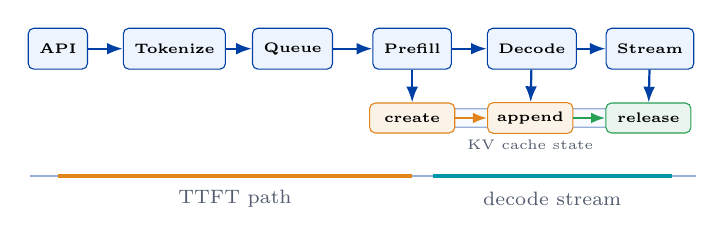
\begin{tikzpicture}[
    x=1cm,y=1cm,
    stage/.style={rounded corners=2pt, draw=HUSTBlue, fill=HUSTLight, minimum height=0.52cm, inner xsep=4pt, align=center, font=\tiny\bfseries},
    state/.style={rounded corners=2pt, draw=HUSTOrange, fill=HUSTOrange!10, minimum width=1.08cm, minimum height=0.38cm, align=center, font=\tiny\bfseries},
    lane/.style={rounded corners=2pt, draw=HUSTLine, fill=HUSTLight!45, minimum height=0.18cm},
    arrow/.style={-{Latex[length=2.0mm]}, thick, draw=HUSTBlue},
    kvflow/.style={-{Latex[length=1.8mm]}, thick, draw=HUSTOrange}
  ]
    \foreach \x/\name/\lab in {0/api/API,1.48/tok/Tokenize,2.98/queue/Queue,4.50/pre/Prefill,6.02/dec/Decode,7.52/stream/Stream} {
      \node[stage] (\name) at (\x,0) {\lab};
    }
    \foreach \a/\b in {api/tok,tok/queue,queue/pre,pre/dec,dec/stream} {\draw[arrow] (\a) -- (\b);}
    \node[lane, minimum width=3.95cm] at (6.00,-0.88) {};
    \node[state] (kv0) at (4.50,-0.88) {create};
    \node[state] (kv1) at (6.00,-0.88) {append};
    \node[state, draw=HUSTGreen, fill=HUSTGreen!10] (rel) at (7.50,-0.88) {release};
    \node[font=\tiny, text=HUSTGray] at (6.00,-1.22) {KV cache state};
    \draw[arrow] (pre) -- (kv0);
    \draw[arrow] (dec) -- (kv1);
    \draw[arrow] (stream) -- (rel);
    \draw[kvflow] (kv0) -- (kv1);
    \draw[kvflow, draw=HUSTGreen] (kv1) -- (rel);
    \draw[HUSTLine, thick] (-0.35,-1.62) -- (8.10,-1.62);
    \draw[HUSTOrange, ultra thick] (0,-1.62) -- (4.50,-1.62);
    \draw[HUSTCyan, ultra thick] (4.76,-1.62) -- (7.80,-1.62);
    \node[font=\scriptsize, text=HUSTGray] at (2.25,-1.90) {TTFT path};
    \node[font=\scriptsize, text=HUSTGray] at (6.28,-1.90) {decode stream};
  \end{tikzpicture}
  \vspace{0.35cm}
  \begin{itemize}
    \item TTFT is dominated by queueing and prefill.
    \item Later token latency is dominated by decode scheduling and KV residency.
  \end{itemize}
\end{frame}

\begin{frame}{Prefill and decode are different workloads}
  \begin{columns}[T,totalwidth=\textwidth]
    \begin{column}{0.48\textwidth}
      \begin{block}{Prefill}
        \begin{itemize}
          \item Reads the whole prompt.
          \item More compute intensive.
          \item Determines first-token latency.
          \item Becomes expensive with long context and RAG.
        \end{itemize}
      \end{block}
    \end{column}
    \begin{column}{0.48\textwidth}
      \begin{block}{Decode}
        \begin{itemize}
          \item Generates one or a few tokens per iteration.
          \item Lighter per step, but repeated many times.
          \item Relies on KV cache staying alive.
          \item Sensitive to scheduling jitter.
        \end{itemize}
      \end{block}
    \end{column}
  \end{columns}
  \vspace{0.3cm}
  \key{They expose different bottlenecks and need different optimization paths.}
\end{frame}

\begin{frame}{Example request: ``Explain transformer attention''}
  \begin{columns}[T,totalwidth=\textwidth]
    \begin{column}{0.52\textwidth}
      \begin{itemize}
        \item Prompt: 600 tokens.
        \item Output: 120 tokens.
        \item Prefill: one relatively heavy pass.
        \item Decode: 120 small iterations.
      \end{itemize}
    \end{column}
    \begin{column}{0.46\textwidth}
      \centering
      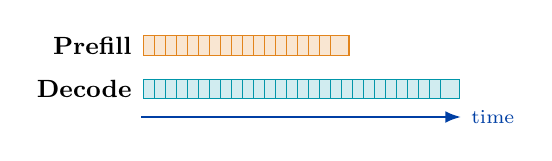
\begin{tikzpicture}[x=0.14cm,y=0.55cm]
        \node[anchor=east,font=\small\bfseries] at (0,1) {Prefill};
        \foreach \i in {1,...,18} {
          \node[draw=HUSTOrange, fill=HUSTOrange!20, minimum width=0.13cm, minimum height=0.25cm] at (\i,1) {};
        }
        \node[anchor=east,font=\small\bfseries] at (0,0) {Decode};
        \foreach \i in {1,...,28} {
          \node[draw=HUSTCyan, fill=HUSTCyan!18, minimum width=0.08cm, minimum height=0.20cm] at (\i,0) {};
        }
        \draw[-{Latex[length=2mm]}, thick, HUSTBlue] (0,-0.65) -- (29,-0.65) node[right,font=\scriptsize] {time};
      \end{tikzpicture}
    \end{column}
  \end{columns}
  \vspace{0.32cm}
  \begin{block}{Observation}
    A user feels both the wait before the first token and the smoothness of the stream afterwards.
  \end{block}
\end{frame}

\begin{frame}{Service metrics}
  \small
  \begin{tabularx}{\textwidth}{>{\bfseries\raggedright\arraybackslash}p{2.35cm}Y}
    \toprule
    Metric & Meaning \\
    \midrule
    TTFT & Time to first token. Strongly affected by queueing and prefill. \\
    TPOT / ITL & Time per output token. Indicates decode steady-state behavior. \\
    Throughput & Tokens/sec or requests/sec. Useful but can hide tail latency. \\
    Goodput & Useful throughput under a latency target. Often better for online services. \\
    P95 / P99 & Tail latency. Important for multi-tenant and bursty workloads. \\
    \bottomrule
  \end{tabularx}
  \vspace{0.25cm}
  \begin{block}{Metric set}
    A serving result is clearest when throughput, latency, tail behavior, and configuration are reported together.
  \end{block}
\end{frame}

\begin{frame}{Where latency is spent}
  \begin{columns}[T,totalwidth=\textwidth]
    \begin{column}{0.48\textwidth}
      \begin{block}{Before the first token}
        \begin{itemize}
          \item Queueing and admission.
          \item Tokenization and request validation.
          \item Prefill over the input context.
          \item KV allocation and graph path selection.
        \end{itemize}
      \end{block}
    \end{column}
    \begin{column}{0.48\textwidth}
      \begin{block}{After the first token}
        \begin{itemize}
          \item Decode iterations.
          \item Batch reshaping.
          \item KV page lookup and residency.
          \item Stream backpressure and tail behavior.
        \end{itemize}
      \end{block}
    \end{column}
  \end{columns}
  \vspace{0.25cm}
  \term{The same request contributes to different bottlenecks at different times.}
\end{frame}

\breakpage
  {Session 2 resumes with scheduling, continuous batching, and KV state.}
  {Keep three objects in mind: the candidate requests, the token budget, and the free KV blocks.}

\topicsectionpage{Part III. Scheduling and State Management}{Continuous batching, KV cache, and stateful execution}

\begin{frame}{Why scheduling comes first}
  \begin{block}{Scheduling tension}
    Online serving must continuously organize requests with very different lengths into efficient batches.
  \end{block}
  \begin{itemize}
    \item Bigger batches improve device utilization.
    \item Bigger batches may also make new users wait longer.
    \item Long requests keep KV state alive for many iterations.
    \item Short requests need low waiting time even when long requests are active.
  \end{itemize}
\end{frame}

\begin{frame}{Head-of-line blocking in mixed workloads}
  \centering
  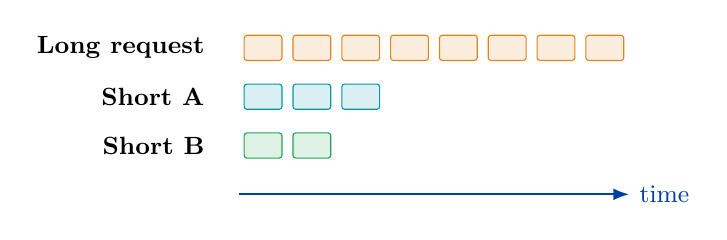
\begin{tikzpicture}[x=0.62cm,y=0.62cm]
    \foreach \r/\name/\len/\col in {0/Long request/8/HUSTOrange,1/Short A/3/HUSTCyan,2/Short B/2/HUSTGreen} {
      \node[anchor=east,font=\small\bfseries] at (0,-\r) {\name};
      \foreach \i in {1,...,\len} {
        \node[draw=\col, fill=\col!15, minimum width=0.48cm, minimum height=0.32cm, rounded corners=1pt] at (\i,-\r) {};
      }
    }
    \draw[-{Latex[length=2mm]}, thick, HUSTBlue] (0.5,-3.0) -- (8.5,-3.0) node[right,font=\small] {time};
  \end{tikzpicture}
  \vspace{0.3cm}
  \begin{itemize}
    \item If the system waits for the whole request to finish, short requests may wait unnecessarily.
    \item Average throughput may look acceptable while TTFT and P99 degrade.
  \end{itemize}
\end{frame}

\begin{frame}{Request-level vs. iteration-level scheduling}
  \small
  \begin{tabularx}{\textwidth}{>{\bfseries\raggedright\arraybackslash}p{2.4cm}YY}
    \toprule
    Granularity & Benefit & Risk \\
    \midrule
    Request & Simple implementation & Poor ability to insert new requests during generation \\
    Iteration & Rebuild batch after each decode round & Needs careful state tracking and KV management \\
    Token & Maximum flexibility & High metadata and synchronization overhead \\
    \bottomrule
  \end{tabularx}
  \vspace{0.28cm}
  \begin{block}{Orca-style intuition}
    Move the scheduling decision from the request boundary to the generation-iteration boundary.
  \end{block}
\end{frame}

\begin{frame}{Continuous batching}
  \centering
  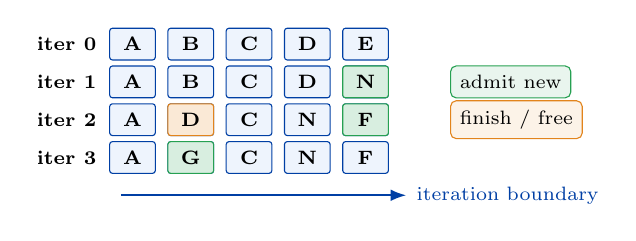
\begin{tikzpicture}[
    x=0.74cm,y=0.48cm,
    slot/.style={draw=HUSTBlue, fill=HUSTLight, minimum width=0.58cm, minimum height=0.30cm, rounded corners=1pt, font=\scriptsize\bfseries},
    new/.style={draw=HUSTGreen, fill=HUSTGreen!18, minimum width=0.58cm, minimum height=0.30cm, rounded corners=1pt, font=\scriptsize\bfseries},
    done/.style={draw=HUSTOrange, fill=HUSTOrange!18, minimum width=0.58cm, minimum height=0.30cm, rounded corners=1pt, font=\scriptsize\bfseries}
  ]
    \foreach \t/\label in {0/iter 0,1/iter 1,2/iter 2,3/iter 3} {
      \node[anchor=east,font=\scriptsize\bfseries] at (-0.45,-\t) {\label};
    }
    \foreach \x/\r in {0/A,1/B,2/C,3/D,4/E} {\node[slot] at (\x,0) {\r};}
    \foreach \x/\r in {0/A,1/B,2/C,3/D,4/N} {\node[slot] at (\x,-1) {\r};}
    \node[new] at (4,-1) {N};
    \foreach \x/\r in {0/A,1/D,2/C,3/N,4/F} {\node[slot] at (\x,-2) {\r};}
    \node[done] at (1,-2) {D};
    \node[new] at (4,-2) {F};
    \foreach \x/\r in {0/A,1/G,2/C,3/N,4/F} {\node[slot] at (\x,-3) {\r};}
    \node[new] at (1,-3) {G};
    \draw[-{Latex[length=2mm]}, thick, HUSTBlue] (-0.2,-4.0) -- (4.7,-4.0) node[right,font=\scriptsize] {iteration boundary};
    \node[draw=HUSTGreen, fill=HUSTGreen!10, rounded corners=2pt, font=\scriptsize, anchor=west] at (5.45,-1.0) {admit new};
    \node[draw=HUSTOrange, fill=HUSTOrange!10, rounded corners=2pt, font=\scriptsize, anchor=west] at (5.45,-2.0) {finish / free};
  \end{tikzpicture}
  \vspace{0.25cm}
  \begin{itemize}
    \item New requests can enter when old requests finish.
    \item The price is that every active request needs its own state tracked across iterations.
  \end{itemize}
\end{frame}

\begin{frame}{Worked scheduler example: two budgets, three requests}
  \begin{block}{This iteration has two hard limits}
    Token budget \(=8\); free KV blocks \(=3\).
  \end{block}
  \begin{center}
    \begin{tabular}{lcc}
      \toprule
      Request & Tokens needed & KV blocks needed \\
      \midrule
      A & 4 & 2 \\
      B & 3 & 1 \\
      C & 5 & 3 \\
      \bottomrule
    \end{tabular}
  \end{center}
  \vspace{0.2cm}
  \term{Question: which pairs fit both budgets?}
\end{frame}

\begin{frame}{Check every candidate pair}
  \begin{enumerate}
    \item \(A+B=(7\text{ tokens},3\text{ blocks})\): feasible.
    \item \(A+C=(9\text{ tokens},5\text{ blocks})\): exceeds both budgets.
    \item \(B+C=(8\text{ tokens},4\text{ blocks})\): token budget fits, KV budget does not.
  \end{enumerate}
  \vspace{0.28cm}
  \begin{block}{Result}
    \(A+B\) is the only feasible pair. Hard constraints define the feasible set; priority and fairness choose among feasible options.
  \end{block}
\end{frame}

\begin{frame}{Feasible does not automatically mean fair}
  \begin{block}{Follow-up scenario}
    Request C has waited for two seconds, while A and B have just arrived.
  \end{block}
  \begin{itemize}
    \item Repeatedly choosing short requests may improve immediate throughput.
    \item The long-waiting request may starve.
    \item Aging, reservations, or SLO-aware priority can bound waiting time.
    \item The evaluation must report throughput, TTFT distribution, TPOT, and maximum wait.
  \end{itemize}
\end{frame}

\begin{frame}{Scheduling is not isolated}
  \centering
  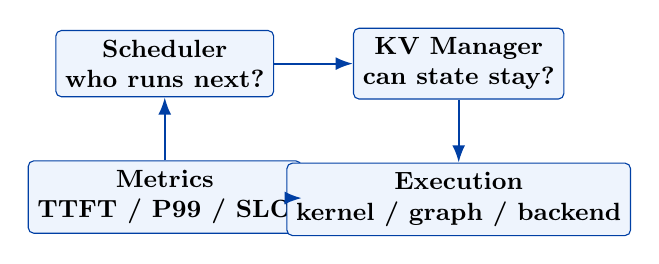
\begin{tikzpicture}[
    box/.style={rounded corners=2pt, draw=HUSTBlue, fill=HUSTLight, minimum width=2.25cm, minimum height=0.74cm, align=center, font=\small\bfseries},
    arrow/.style={-{Latex[length=2.2mm]}, thick, draw=HUSTBlue}
  ]
    \node[box] (sched) {Scheduler\\who runs next?};
    \node[box, right=1.0cm of sched] (kv) {KV Manager\\can state stay?};
    \node[box, below=0.8cm of sched] (metric) {Metrics\\TTFT / P99 / SLO};
    \node[box, below=0.8cm of kv] (exec) {Execution\\kernel / graph / backend};
    \draw[arrow] (sched) -- (kv);
    \draw[arrow] (kv) -- (exec);
    \draw[arrow] (exec) -- (metric);
    \draw[arrow] (metric) -- (sched);
  \end{tikzpicture}
  \vspace{0.35cm}
  \begin{block}{Coupling point}
    Scheduling decisions, KV residency, execution path, and service metrics form one feedback loop.
  \end{block}
\end{frame}

\begin{frame}{Why KV cache is central}
  \begin{itemize}
    \item KV grows with context length and concurrency.
    \item It must stay resident across many decode iterations.
    \item It limits effective batch size.
    \item It turns every active request into a stateful object.
    \item Once prefix reuse is enabled, KV becomes a shared resource.
  \end{itemize}
  \vspace{0.35cm}
  \begin{center}
    \Large\term{KV cache is not an implementation detail. It is a first-class system resource.}
  \end{center}
\end{frame}

\begin{frame}{Worked KV example: bytes per token}
  \begin{block}{Model configuration}
    \(L=32\) layers, \(H_{\mathrm{kv}}=8\) KV heads,
    \(d_{\mathrm{head}}=128\), FP16 \(=2\) bytes per value.
  \end{block}
  \[
    \text{KV bytes/token}
    =2\times L\times H_{\mathrm{kv}}\times d_{\mathrm{head}}\times\text{bytes}
  \]
  \[
    =2\times32\times8\times128\times2
    =131{,}072\text{ bytes}
    =128\text{ KiB}.
  \]
  \begin{itemize}
    \item The first factor of two means one \(K\) and one \(V\).
    \item 100 new tokens add approximately \(12.5\) MiB per request.
  \end{itemize}
\end{frame}

\begin{frame}{Worked paging example: 40 tokens, block size 16}
  \begin{enumerate}
    \item Tokens 1--16 fill logical block 0.
    \item Tokens 17--32 fill logical block 1.
    \item Tokens 33--40 require logical block 2.
  \end{enumerate}
  \[
    \text{blocks}=\left\lceil\frac{40}{16}\right\rceil=3,
    \qquad
    \text{unused slots}=3\times16-40=8.
  \]
  \begin{block}{Interpretation}
    Paging avoids a contiguous 40-token allocation, but capacity still grows in block-sized units.
  \end{block}
\end{frame}

\begin{frame}{KV cache lifecycle}
  \centering
  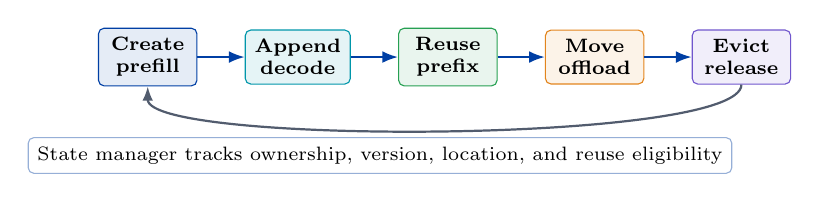
\begin{tikzpicture}[
    node distance=0.60cm,
    kvblue/.style={rounded corners=2pt, draw=HUSTBlue, fill=HUSTBlue!10, minimum width=1.25cm, minimum height=0.55cm, align=center, font=\scriptsize\bfseries},
    kvcyan/.style={rounded corners=2pt, draw=HUSTCyan, fill=HUSTCyan!10, minimum width=1.25cm, minimum height=0.55cm, align=center, font=\scriptsize\bfseries},
    kvgreen/.style={rounded corners=2pt, draw=HUSTGreen, fill=HUSTGreen!10, minimum width=1.25cm, minimum height=0.55cm, align=center, font=\scriptsize\bfseries},
    kvorange/.style={rounded corners=2pt, draw=HUSTOrange, fill=HUSTOrange!10, minimum width=1.25cm, minimum height=0.55cm, align=center, font=\scriptsize\bfseries},
    kvpurple/.style={rounded corners=2pt, draw=HUSTPurple, fill=HUSTPurple!10, minimum width=1.25cm, minimum height=0.55cm, align=center, font=\scriptsize\bfseries},
    arrow/.style={-{Latex[length=2.0mm]}, thick, draw=HUSTBlue}
  ]
    \node[kvblue] (create) at (0,0) {Create\\prefill};
    \node[kvcyan, right=of create] (append) {Append\\decode};
    \node[kvgreen, right=of append] (reuse) {Reuse\\prefix};
    \node[kvorange, right=of reuse] (move) {Move\\offload};
    \node[kvpurple, right=of move] (evict) {Evict\\release};
    \foreach \a/\b in {create/append,append/reuse,reuse/move,move/evict} {\draw[arrow] (\a) -- (\b);}
    \draw[-{Latex[length=1.8mm]}, thick, draw=HUSTGray] (evict.south) .. controls +(0,-0.75) and +(0,-0.75) .. node[below,font=\scriptsize,text=HUSTGray] {free block for another request} (create.south);
    \node[rounded corners=2pt, draw=HUSTLine, fill=white, minimum width=5.8cm, minimum height=0.44cm, font=\scriptsize] at (2.95,-1.25) {State manager tracks ownership, version, location, and reuse eligibility};
  \end{tikzpicture}
  \vspace{0.32cm}
  \begin{block}{Design point}
    Each optimization changes one lifecycle step and may shift cost elsewhere.
  \end{block}
\end{frame}

\begin{frame}{Request state and physical KV state are different}
  \begin{block}{Example: request R17}
    \[
      \texttt{WAITING}
      \rightarrow
      \texttt{RUNNING}
      \rightarrow
      \texttt{PREEMPTED}
      \rightarrow
      \texttt{RUNNING}
      \rightarrow
      \texttt{FINISHED}.
    \]
  \end{block}
  \begin{itemize}
    \item Logical state records tokens, phase, and progress.
    \item Physical state records devices, blocks, addresses, and in-flight operations.
    \item After preemption, the same logical tokens may resume on different physical blocks.
    \item Release is safe only after ownership, references, and asynchronous use are resolved.
  \end{itemize}
\end{frame}

\begin{frame}{Shared prefix example: reference count prevents early reuse}
  \begin{block}{Initial state}
    Requests R17 and R18 share prefix block P3, so \(\operatorname{refcount}(P3)=2\).
  \end{block}
  \begin{enumerate}
    \item R17 is cancelled: the count drops from 2 to 1.
    \item P3 cannot return to the free list because R18 still reads it.
    \item R18 finishes: the count drops from 1 to 0.
    \item After in-flight device reads complete, P3 may be reclaimed.
  \end{enumerate}
  \vspace{0.2cm}
  \key{Reference count handles sharing; a device event or fence handles asynchronous completion.}
\end{frame}

\begin{frame}{Why contiguous allocation breaks down}
  \begin{columns}[T,totalwidth=\textwidth]
    \begin{column}{0.50\textwidth}
      \begin{block}{If KV must be contiguous}
        \begin{itemize}
          \item Dynamic lengths create fragmentation.
          \item Reserving too much wastes memory.
          \item Reserving too little causes failures.
        \end{itemize}
      \end{block}
    \end{column}
    \begin{column}{0.50\textwidth}
      \begin{block}{Paged idea}
        \begin{itemize}
          \item Split KV into blocks.
          \item Map logical sequence to physical pages.
          \item Let the scheduler manage more dynamic requests.
        \end{itemize}
      \end{block}
    \end{column}
  \end{columns}
\end{frame}

\begin{frame}{Paged KV: a visual analogy}
  \centering
  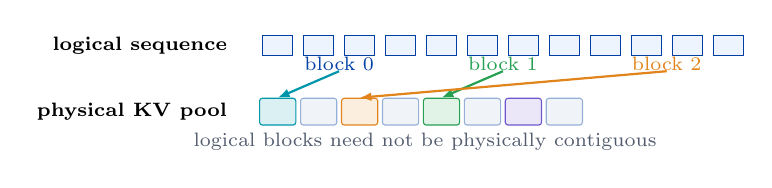
\begin{tikzpicture}[x=0.52cm,y=0.48cm,
    token/.style={draw=HUSTBlue, fill=HUSTLight, minimum width=0.38cm, minimum height=0.26cm},
    pagecyan/.style={draw=HUSTCyan, fill=HUSTCyan!14, minimum width=0.46cm, minimum height=0.34cm, rounded corners=1pt},
    pagegreen/.style={draw=HUSTGreen, fill=HUSTGreen!14, minimum width=0.46cm, minimum height=0.34cm, rounded corners=1pt},
    pageorange/.style={draw=HUSTOrange, fill=HUSTOrange!14, minimum width=0.46cm, minimum height=0.34cm, rounded corners=1pt},
    pagepurple/.style={draw=HUSTPurple, fill=HUSTPurple!14, minimum width=0.46cm, minimum height=0.34cm, rounded corners=1pt},
    pagefree/.style={draw=HUSTLine, fill=HUSTLine!14, minimum width=0.46cm, minimum height=0.34cm, rounded corners=1pt}
  ]
    \node[anchor=east,font=\scriptsize\bfseries] at (0,1.6) {logical sequence};
    \foreach \i in {1,...,12} {\node[token] (t\i) at (\i,1.6) {};}
    \node[font=\scriptsize,text=HUSTBlue] at (2.5,1.12) {block 0};
    \node[font=\scriptsize,text=HUSTGreen] at (6.5,1.12) {block 1};
    \node[font=\scriptsize,text=HUSTOrange] at (10.5,1.12) {block 2};
    \node[anchor=east,font=\scriptsize\bfseries] at (0,-0.15) {physical KV pool};
    \node[pagecyan] (p0) at (1,-0.15) {};
    \node[pagefree] (free1) at (2,-0.15) {};
    \node[pageorange] (p2) at (3,-0.15) {};
    \node[pagefree] (free2) at (4,-0.15) {};
    \node[pagegreen] (p1) at (5,-0.15) {};
    \node[pagefree] (free3) at (6,-0.15) {};
    \node[pagepurple] (p3) at (7,-0.15) {};
    \node[pagefree] (free4) at (8,-0.15) {};
    \draw[-{Latex[length=1.5mm]}, HUSTCyan, thick] (2.5,0.92) -- (p0.north);
    \draw[-{Latex[length=1.5mm]}, HUSTGreen, thick] (6.5,0.92) -- (p1.north);
    \draw[-{Latex[length=1.5mm]}, HUSTOrange, thick] (10.5,0.92) -- (p2.north);
    \node[font=\scriptsize,text=HUSTGray] at (4.6,-0.95) {logical blocks need not be physically contiguous};
  \end{tikzpicture}
  \vspace{0.35cm}
  \begin{block}{System effect}
    PagedAttention-style management reduces memory waste, supports dynamic batching, and creates a handle for reuse, migration, and multi-level KV storage.
  \end{block}
\end{frame}

\begin{frame}{Sharing KV: a small RAG example}
  \begin{columns}[T,totalwidth=\textwidth]
    \begin{column}{0.52\textwidth}
      \begin{itemize}
        \item User A asks about a course policy.
        \item User B asks a different question about the same policy document.
        \item Both prompts include the same retrieved paragraph.
      \end{itemize}
      \vspace{0.2cm}
      \key{Opportunity}: reuse the expensive state for the shared segment.
    \end{column}
    \begin{column}{0.46\textwidth}
      \centering
      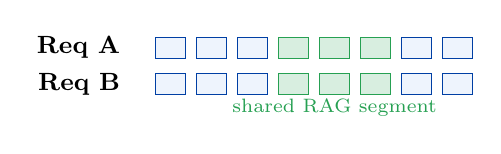
\begin{tikzpicture}[x=0.52cm,y=0.46cm]
        \foreach \r/\name in {0/A,1/B} {
          \node[anchor=east,font=\small\bfseries] at (0,-\r) {Req \name};
          \foreach \i in {1,...,8} {
            \pgfmathtruncatemacro{\shared}{(\i>=4 && \i<=6) ? 1 : 0}
            \ifnum\shared=1
              \node[draw=HUSTGreen, fill=HUSTGreen!18, minimum width=0.38cm, minimum height=0.26cm] at (\i,-\r) {};
            \else
              \node[draw=HUSTBlue, fill=HUSTLight, minimum width=0.38cm, minimum height=0.26cm] at (\i,-\r) {};
            \fi
          }
        }
        \node[font=\scriptsize, text=HUSTGreen] at (5,-1.65) {shared RAG segment};
      \end{tikzpicture}
    \end{column}
  \end{columns}
  \vspace{0.28cm}
  \begin{block}{But sharing has a contract}
    Version, parameters, permissions, and semantic boundaries must match.
  \end{block}
\end{frame}

\begin{frame}{State decisions made by the runtime}
  \small
  \begin{tabularx}{\textwidth}{>{\bfseries\raggedright\arraybackslash}p{2.1cm}YY}
    \toprule
    Decision & Local benefit & System cost \\
    \midrule
    Keep & Avoid recomputation & Occupies memory and limits new batches \\
    Reuse & Save prefill work & Requires matching, validation, and ownership checks \\
    Move & Release device memory & Adds transfer latency and coordination \\
    Evict & Admit urgent work & May trigger recomputation later \\
    \bottomrule
  \end{tabularx}
  \vspace{0.28cm}
  \begin{block}{Scheduling view}
    The scheduler is no longer choosing only which request runs next; it also chooses which state remains valuable.
  \end{block}
\end{frame}

\begin{frame}{Checkpoint: make one scheduling decision}
  \begin{block}{Given}
    Token budget \(=10\), free blocks \(=4\). Request D needs \((6,2)\), E needs \((4,2)\), and F needs \((3,3)\).
  \end{block}
  \begin{enumerate}
    \item List all feasible request pairs.
    \item Choose one pair if F has the oldest deadline.
    \item State which metric could become worse because of your choice.
    \item Name the event fields needed to explain the decision later.
  \end{enumerate}
  \smallnote{A complete answer separates feasibility, policy, expected effect, and evidence.}
\end{frame}

\topicsectionpage{Part IV. Modern Workloads and Heterogeneous Execution}{Long context, RAG, MoE, agents, and accelerator dynamics}

\begin{frame}{KV pressure changes scheduling}
  \begin{block}{Scenario}
    The GPU/NPU memory is almost full. A new high-priority request arrives.
  \end{block}
  \begin{columns}[T,totalwidth=\textwidth]
    \begin{column}{0.34\textwidth}
      \textbf{\textcolor{HUSTBlue}{Option 1}}\\
      Keep all KV, reject or delay the new request.
    \end{column}
    \begin{column}{0.34\textwidth}
      \textbf{\textcolor{HUSTBlue}{Option 2}}\\
      Preempt one request and keep its KV elsewhere.
    \end{column}
    \begin{column}{0.30\textwidth}
      \textbf{\textcolor{HUSTBlue}{Option 3}}\\
      Drop KV and recompute later.
    \end{column}
  \end{columns}
  \vspace{0.35cm}
  \key{Scheduling now includes a state-utility decision.}
\end{frame}

\begin{frame}{New forms of intermediate state}
  \small
  \begin{tabularx}{\textwidth}{>{\bfseries\raggedright\arraybackslash}p{2.5cm}YY}
    \toprule
    State form & Where it comes from & System challenge \\
    \midrule
    KV blocks & Long context and continuous batching & Memory pressure, fragmentation, eviction \\
    Prefix / segment & System prompts, RAG, templates & Matching, consistency, reuse cost \\
    Draft state & Speculative decoding & Branching, rollback, commit \\
    Agent state & Tool calls and multi-turn memory & Cross-step propagation, isolation \\
    \bottomrule
  \end{tabularx}
  \vspace{0.28cm}
  \begin{block}{Research trend}
    Intermediate state is becoming a managed resource, not a temporary tensor.
  \end{block}
\end{frame}

\begin{frame}{Long context and RAG}
  \begin{itemize}
    \item Longer prompts amplify prefill cost.
    \item RAG makes input length and overlap more variable.
    \item Similar documents create reuse opportunities.
    \item The benefit depends on matching cost, memory pressure, and latency targets.
  \end{itemize}
  \vspace{0.35cm}
  \begin{block}{Example}
    A university assistant may answer 100 different questions using the same handbook. Blindly recomputing the handbook prefix wastes prefill work.
  \end{block}
\end{frame}

\begin{frame}{MoE: routing is dynamic}
  \begin{block}{What changes with MoE?}
    Each token may activate different experts, and the expert load can change from token to token.
  \end{block}
  \begin{columns}[T,totalwidth=\textwidth]
    \begin{column}{0.48\textwidth}
      \begin{itemize}
        \item Expert load imbalance.
        \item Expert parallel communication.
        \item Expert offloading and residency.
        \item Dynamic expert-to-device mapping.
      \end{itemize}
    \end{column}
    \begin{column}{0.48\textwidth}
      \centering
      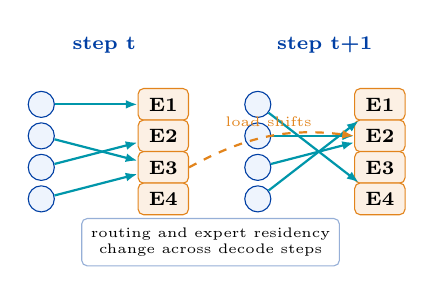
\begin{tikzpicture}[
        tok/.style={circle, draw=HUSTBlue, fill=HUSTLight, minimum size=0.32cm, font=\tiny},
        exp/.style={rounded corners=2pt, draw=HUSTOrange, fill=HUSTOrange!12, minimum width=0.64cm, minimum height=0.32cm, font=\scriptsize\bfseries},
        route/.style={-{Latex[length=1.5mm]}, thick, draw=HUSTCyan},
        move/.style={-{Latex[length=1.5mm]}, thick, dashed, draw=HUSTOrange}
      ]
        \node[font=\scriptsize\bfseries,text=HUSTBlue] at (0.8,0.35) {step t};
        \node[font=\scriptsize\bfseries,text=HUSTBlue] at (3.6,0.35) {step t+1};
        \foreach \i in {1,...,4} {\node[tok] (a\i) at (0,-0.40*\i) {};}
        \foreach \j in {1,...,4} {\node[exp] (e\j) at (1.55,-0.40*\j) {E\j};}
        \foreach \i in {1,...,4} {\node[tok] (b\i) at (2.75,-0.40*\i) {};}
        \foreach \j in {1,...,4} {\node[exp] (f\j) at (4.30,-0.40*\j) {E\j};}
        \draw[route] (a1) -- (e1); \draw[route] (a2) -- (e3); \draw[route] (a3) -- (e2); \draw[route] (a4) -- (e3);
        \draw[route] (b1) -- (f4); \draw[route] (b2) -- (f2); \draw[route] (b3) -- (f2); \draw[route] (b4) -- (f1);
        \draw[move] (e3.east) to[bend left=18] node[above,font=\tiny,text=HUSTOrange] {load shifts} (f2.west);
        \node[rounded corners=2pt, draw=HUSTLine, fill=white, font=\tiny, align=center] at (2.15,-2.15) {routing and expert residency\\change across decode steps};
      \end{tikzpicture}
    \end{column}
  \end{columns}
  \vspace{0.25cm}
  \key{Challenge}: dynamic expert mapping conflicts with stable graph replay requirements.
\end{frame}

\begin{frame}{Agents: one request becomes a workflow}
  \centering
  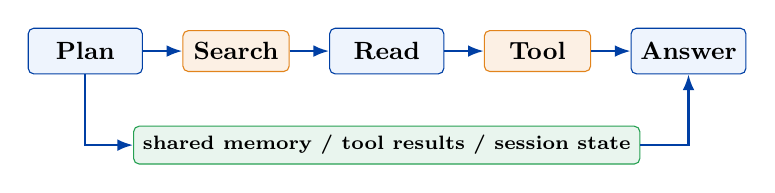
\begin{tikzpicture}[
    node distance=0.5cm,
    agentstep/.style={rounded corners=2pt, draw=HUSTBlue, fill=HUSTLight, minimum width=1.45cm, minimum height=0.58cm, align=center, font=\small\bfseries},
    tool/.style={rounded corners=2pt, draw=HUSTOrange, fill=HUSTOrange!12, minimum width=1.35cm, minimum height=0.52cm, align=center, font=\small\bfseries},
    arrow/.style={-{Latex[length=2mm]}, thick, draw=HUSTBlue}
  ]
    \node[agentstep] (plan) {Plan};
    \node[tool, right=of plan] (search) {Search};
    \node[agentstep, right=of search] (read) {Read};
    \node[tool, right=of read] (code) {Tool};
    \node[agentstep, right=of code] (answer) {Answer};
    \draw[arrow] (plan) -- (search);
    \draw[arrow] (search) -- (read);
    \draw[arrow] (read) -- (code);
    \draw[arrow] (code) -- (answer);
    \node[draw=HUSTGreen, fill=HUSTGreen!10, rounded corners=2pt, below=0.65cm of read, minimum width=4.0cm, minimum height=0.45cm, font=\scriptsize\bfseries] (mem) {shared memory / tool results / session state};
    \draw[arrow] (plan) |- (mem);
    \draw[arrow] (mem) -| (answer);
  \end{tikzpicture}
  \vspace{0.35cm}
  \begin{itemize}
    \item Agent requests create intermediate state across multiple steps.
    \item Scheduling, caching, and isolation now span a workflow, not a single sequence.
  \end{itemize}
\end{frame}

\begin{frame}{Many reuse mechanisms, one selection problem}
  \begin{block}{Selection space}
    APC, prompt cache, CacheBlend, LMCache, and other mechanisms may all help, but each has different cost and applicability.
  \end{block}
  \begin{columns}[T,totalwidth=\textwidth]
    \begin{column}{0.47\textwidth}
      \begin{itemize}
        \item Timing of reuse attempts.
        \item Request and segment selection.
        \item Mechanism selection.
        \item Detection cost versus recomputation cost.
      \end{itemize}
    \end{column}
    \begin{column}{0.49\textwidth}
      \centering
      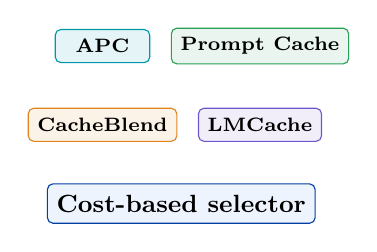
\begin{tikzpicture}
        \node[rounded corners=2pt, draw=HUSTCyan, fill=HUSTCyan!10, minimum width=1.2cm, minimum height=0.42cm, font=\scriptsize\bfseries] at (0,1) {APC};
        \node[rounded corners=2pt, draw=HUSTGreen, fill=HUSTGreen!10, minimum width=1.2cm, minimum height=0.42cm, font=\scriptsize\bfseries] at (2,1) {Prompt Cache};
        \node[rounded corners=2pt, draw=HUSTOrange, fill=HUSTOrange!10, minimum width=1.2cm, minimum height=0.42cm, font=\scriptsize\bfseries] at (0,0) {CacheBlend};
        \node[rounded corners=2pt, draw=HUSTPurple, fill=HUSTPurple!10, minimum width=1.2cm, minimum height=0.42cm, font=\scriptsize\bfseries] at (2,0) {LMCache};
        \node[draw=HUSTBlue, fill=HUSTLight, rounded corners=2pt, minimum width=2.6cm, minimum height=0.5cm, font=\small\bfseries] at (1,-1.0) {Cost-based selector};
      \end{tikzpicture}
    \end{column}
  \end{columns}
\end{frame}

\begin{frame}{Modern workloads change the control surface}
  \small
  \begin{tabularx}{\textwidth}{>{\bfseries\raggedright\arraybackslash}p{2.2cm}YY}
    \toprule
    Workload & New pressure & Control point \\
    \midrule
    Long context & Heavy prefill and large KV & Prefix reuse, paging, admission \\
    RAG & Shared but imperfect context overlap & Segment matching and validation \\
    MoE & Dynamic expert load and residency & Routing, expert placement, graph path \\
    Agents & Multi-step state and tool outputs & Workflow scheduling and isolation \\
    \bottomrule
  \end{tabularx}
  \vspace{0.28cm}
  \begin{block}{Teaching point}
    Modern inference systems optimize a moving service workflow, not a single static model invocation.
  \end{block}
\end{frame}

\begin{frame}{Platform differences are system differences}
  \begin{itemize}
    \item Operator libraries differ.
    \item Graph execution and compilation behavior differ.
    \item Interconnect and host-device paths differ.
    \item Profiling and debugging tools differ.
    \item Default precision and fallback behavior differ.
  \end{itemize}
  \vspace{0.32cm}
  \begin{block}{Takeaway}
    A GPU optimization is a hypothesis, not a guaranteed solution, on NPU/DCU/XPU platforms.
  \end{block}
\end{frame}

\begin{frame}{Three levels of adaptation}
  \begin{enumerate}
    \item \term{Can run}: model loading, basic inference, correct output.
    \item \term{Can optimize}: platform-aware kernels, graph paths, memory and communication.
    \item \term{Can verify}: fair baseline, controlled workload, reproducible metadata.
  \end{enumerate}
  \vspace{0.35cm}
  \begin{block}{Research usually starts at level 2}
    Running is necessary, but optimization and verification are where system research begins.
  \end{block}
\end{frame}

\begin{frame}{Graph replay wants stability; serving wants dynamics}
  \begin{columns}[T,totalwidth=\textwidth]
    \begin{column}{0.50\textwidth}
      \begin{block}{High-performance execution wants}
        \begin{itemize}
          \item Stable shapes
          \item Stable addresses
          \item Stable memory layout
          \item Predictable kernels
        \end{itemize}
      \end{block}
    \end{column}
    \begin{column}{0.50\textwidth}
      \begin{block}{Online serving gives}
        \begin{itemize}
          \item Variable prompt lengths
          \item Dynamic batching
          \item Changing KV pages
          \item MoE routing changes
        \end{itemize}
      \end{block}
    \end{column}
  \end{columns}
  \vspace{0.3cm}
  \key{This conflict is especially visible on graph-oriented accelerator stacks.}
\end{frame}

\begin{frame}{Same FLOPs can produce very different latency}
  \begin{block}{Two kernels each perform 1 GFLOP}
    Kernel A reads 64 MiB from HBM; Kernel B reads 16 MiB.
  \end{block}
  \[
    I_A\approx\frac{10^9}{64\times2^{20}}=14.9\ \text{FLOP/byte},
    \qquad
    I_B\approx59.6\ \text{FLOP/byte}.
  \]
  \begin{itemize}
    \item B has four times the arithmetic intensity.
    \item Under a bandwidth bottleneck, B has a much lower memory-time bound.
    \item FLOPs alone do not determine kernel time or end-to-end time.
  \end{itemize}
\end{frame}

\begin{frame}{A 2x kernel speedup may yield only 1.25x end to end}
  \begin{block}{Profile result}
    The optimized kernel accounts for 40\% of request time; everything else accounts for 60\%.
  \end{block}
  \[
    T_{\text{new}}=0.60+\frac{0.40}{2}=0.80,
    \qquad
    \text{end-to-end speedup}=\frac{1}{0.80}=1.25\times.
  \]
  \begin{itemize}
    \item Local speedup answers whether the mechanism worked.
    \item End-to-end speedup answers whether the user benefited.
    \item A new profile checks whether the bottleneck moved.
  \end{itemize}
\end{frame}

\begin{frame}{Cross-platform correctness starts with a contract}
  \begin{block}{One FP16 output fragment}
    GPU: \([0.5000,-1.2500,2.0000,0.1250]\)\\
    NPU: \([0.5005,-1.2490,1.9980,0.1252]\)
  \end{block}
  \begin{enumerate}
    \item Maximum absolute error is \(0.0020\).
    \item Compare it with a pre-declared tolerance for this dtype and operator.
    \item Separately test masking, boundary shapes, fallback, and multi-step state updates.
  \end{enumerate}
  \vspace{0.2cm}
  \key{Portability means equivalent semantics and observable behavior, not necessarily bitwise identity.}
\end{frame}

\begin{frame}{Measurement checklist}
  \begin{itemize}
    \item End-to-end: TTFT, TPOT, P99, goodput.
    \item Runtime probes: graph hit rate, fallback count, memory allocation failures.
    \item Hardware probes: device utilization, HBM usage, communication time.
    \item Stability probes: variance across runs, tail behavior under bursty load.
  \end{itemize}
  \vspace{0.3cm}
  \begin{block}{Cause separation}
    Is the regression caused by scheduling, memory pressure, graph fallback, communication, or benchmark mismatch?
  \end{block}
\end{frame}

\breakpage
  {Session 3 resumes with heterogeneous execution, evidence, and open engineering.}
  {Keep the comparison matched: same model, shape, dtype, hardware scope, workload, and metric definition.}

\topicsectionpage{Part V. Evidence and Open Engineering Practice}{Benchmarking, reproducibility, and vLLM-HUST workflow}

\begin{frame}{Why benchmark evidence is fragile}
  \begin{itemize}
    \item Same workload name, different token distribution.
    \item Same model name, different precision or parallelism.
    \item Same code path, different backend defaults.
    \item Same throughput, very different tail latency.
    \item Same benchmark, missing metadata.
  \end{itemize}
  \vspace{0.35cm}
  \begin{center}
    \large\term{A benchmark is an evidence chain: workload, setup, baseline, and metrics.}
  \end{center}
\end{frame}

\begin{frame}{Minimum metadata for a credible result}
  \begin{tabularx}{\textwidth}{>{\bfseries\raggedright\arraybackslash}p{2.2cm}Y}
    \toprule
    Category & Must record \\
    \midrule
    Code & Repository, commit, PR, dependency versions \\
    Model & Model ID, dtype, quantization, parallel strategy \\
    Hardware & Device type, number of cards, driver, runtime stack \\
    Service config & Max length, graph/eager mode, cache/offload settings \\
    Workload & Input/output lengths, concurrency, arrival process, data source \\
    Metrics & TTFT, TPOT, P99, throughput, goodput, memory usage \\
    \bottomrule
  \end{tabularx}
\end{frame}

\begin{frame}{Example: a misleading performance trend}
  \begin{columns}[T,totalwidth=\textwidth]
    \begin{column}{0.48\textwidth}
      \centering
      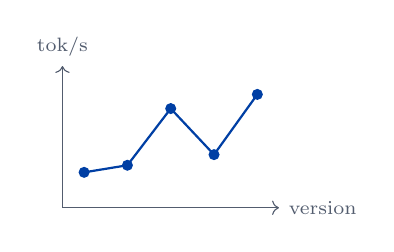
\begin{tikzpicture}[x=0.55cm,y=0.45cm]
        \draw[->, HUSTGray] (0,0) -- (5,0) node[right,font=\scriptsize] {version};
        \draw[->, HUSTGray] (0,0) -- (0,4) node[above,font=\scriptsize] {tok/s};
        \draw[thick, HUSTBlue] (0.5,1.0) -- (1.5,1.2) -- (2.5,2.8) -- (3.5,1.5) -- (4.5,3.2);
        \foreach \x/\y in {0.5/1.0,1.5/1.2,2.5/2.8,3.5/1.5,4.5/3.2} {
          \fill[HUSTBlue] (\x,\y) circle (2pt);
        }
      \end{tikzpicture}
    \end{column}
    \begin{column}{0.48\textwidth}
      \begin{block}{Consistency checks}
        \begin{itemize}
          \item Same model?
          \item Same input/output length?
          \item Same dtype?
          \item Same graph mode?
          \item Same hardware and driver?
        \end{itemize}
      \end{block}
    \end{column}
  \end{columns}
  \vspace{0.25cm}
  \key{A large jump needs attribution: optimization effect or experiment change.}
\end{frame}

\begin{frame}{A controlled A/B result reports a distribution}
  \begin{block}{Hypothesis}
    A fused kernel lowers operator latency for one fixed shape.
  \end{block}
  \begin{itemize}
    \item Hold model, shape, dtype, hardware, version, stream, and timing boundary constant.
    \item Warm up both paths, then measure each path 30 times.
    \item Baseline: median \(12.4\) ms, P95 \(13.1\) ms.
    \item Fused: median \(10.2\) ms, P95 \(10.8\) ms.
  \end{itemize}
  \[
    \text{median speedup}=\frac{12.4}{10.2}\approx1.22\times.
  \]
\end{frame}

\begin{frame}{Do not turn 1.22x microbenchmark gain into a system claim}
  \begin{block}{End-to-end measurement on the same workload}
    Request latency changes from 100 ms to 96 ms.
  \end{block}
  \[
    \text{system speedup}=\frac{100}{96}\approx1.042\times.
  \]
  \begin{itemize}
    \item The operator result is \(1.22\times\).
    \item The user-visible result is about \(4.2\%\).
    \item Profile data explains the gap by showing the optimized operator's time share.
  \end{itemize}
  \term{Report both results, with different labels and scopes.}
\end{frame}

\begin{frame}{From observation to evidence}
  \centering
  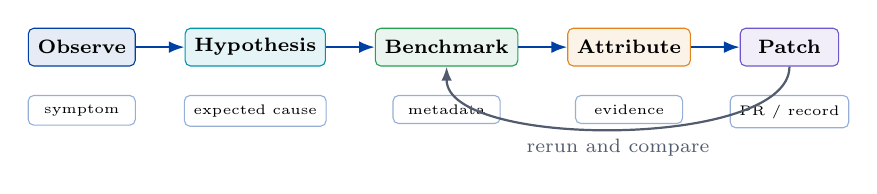
\begin{tikzpicture}[
    node distance=0.62cm,
    evblue/.style={rounded corners=2pt, draw=HUSTBlue, fill=HUSTBlue!10, minimum width=1.25cm, minimum height=0.48cm, align=center, font=\scriptsize\bfseries},
    evcyan/.style={rounded corners=2pt, draw=HUSTCyan, fill=HUSTCyan!10, minimum width=1.25cm, minimum height=0.48cm, align=center, font=\scriptsize\bfseries},
    evgreen/.style={rounded corners=2pt, draw=HUSTGreen, fill=HUSTGreen!10, minimum width=1.25cm, minimum height=0.48cm, align=center, font=\scriptsize\bfseries},
    evorange/.style={rounded corners=2pt, draw=HUSTOrange, fill=HUSTOrange!10, minimum width=1.25cm, minimum height=0.48cm, align=center, font=\scriptsize\bfseries},
    evpurple/.style={rounded corners=2pt, draw=HUSTPurple, fill=HUSTPurple!10, minimum width=1.25cm, minimum height=0.48cm, align=center, font=\scriptsize\bfseries},
    artifact/.style={rounded corners=2pt, draw=HUSTLine, fill=white, minimum width=1.36cm, minimum height=0.34cm, align=center, font=\tiny},
    arrow/.style={-{Latex[length=2mm]}, thick, draw=HUSTBlue}
  ]
    \node[evblue] (obs) at (0,0) {Observe};
    \node[evcyan, right=of obs] (hyp) {Hypothesis};
    \node[evgreen, right=of hyp] (bench) {Benchmark};
    \node[evorange, right=of bench] (attr) {Attribute};
    \node[evpurple, right=of attr] (patch) {Patch};
    \foreach \a/\b in {obs/hyp,hyp/bench,bench/attr,attr/patch} {\draw[arrow] (\a) -- (\b);}
    \node[artifact, below=0.36cm of obs] {symptom};
    \node[artifact, below=0.36cm of hyp] {expected cause};
    \node[artifact, below=0.36cm of bench] {metadata};
    \node[artifact, below=0.36cm of attr] {evidence};
    \node[artifact, below=0.36cm of patch] {PR / record};
    \draw[-{Latex[length=1.8mm]}, thick, draw=HUSTGray] (patch.south) .. controls +(0,-1.05) and +(0,-1.05) .. node[below,font=\scriptsize,text=HUSTGray] {rerun and compare} (bench.south);
  \end{tikzpicture}
  \vspace{0.36cm}
  \begin{block}{Evidence loop}
    A performance claim becomes useful only after the baseline, workload, configuration, and code path are recorded and rerun.
  \end{block}
\end{frame}

\begin{frame}{vLLM-HUST: putting system work into an open workflow}
  \begin{block}{Practice target}
    vLLM-HUST, vLLM-Ascend-HUST, benchmark, and dev-hub repositories organize real inference-system development tasks.
  \end{block}
  \begin{itemize}
    \item Start from an issue, CI failure, benchmark gap, or documentation problem.
    \item Record environment, code path, commands, and failure symptoms.
    \item Submit a small patch or standardized benchmark record.
    \item Use CI, review, and reruns to create maintainable evidence.
  \end{itemize}
\end{frame}

\begin{frame}{Hands-on practice path}
  \begin{itemize}
    \item Define the system path being changed.
    \item Build a minimal reproduction.
    \item Compare against a clear baseline.
    \item Record metadata and known limitations.
    \item Produce a patch, PR, benchmark record, or documentation artifact.
  \end{itemize}
  \vspace{0.25cm}
  \begin{block}{Practice goal}
    Turn a system observation into a reproducible engineering claim.
  \end{block}
\end{frame}

\begin{frame}{Final evidence exercise: fact, inference, decision}
  \begin{block}{Trace summary}
    P99 latency is 1.8 s: queueing 1.1 s, prefill 0.4 s, first decode step 0.2 s, and network 0.1 s.
  \end{block}
  \begin{enumerate}
    \item \textbf{Fact}: queueing accounts for about 61\% of the measured P99 path.
    \item \textbf{Inference}: admission or capacity pressure may dominate.
    \item \textbf{Decision}: record candidate sets, budgets, free blocks, and request ages.
    \item \textbf{Next test}: compare the current policy with an aging-aware policy on a fixed workload.
  \end{enumerate}
\end{frame}

\topicsectionpage{Closing}{Concepts, open questions, and further reading}

\begin{frame}{Six concepts to remember}
  \begin{enumerate}
    \item \term{Attention}: match with \(QK^\top\), then mix visible \(V\) vectors.
    \item \term{Autoregression}: one selected token unlocks the next generation step.
    \item \term{Prefill and decode}: different shapes, timing, and bottlenecks.
    \item \term{Scheduling and KV}: dynamic batches depend on persistent request state.
    \item \term{Heterogeneous execution}: hardware differences reshape the viable path.
    \item \term{Evidence}: matched workloads and complete metadata bound every claim.
  \end{enumerate}
\end{frame}

\begin{frame}{Open research questions}
  \begin{itemize}
    \item Global selection among KV reuse mechanisms.
    \item Boundaries for saving, sharing, or isolating agent intermediate state.
    \item How can MoE routing coexist with high-performance graph replay?
    \item Which GPU serving lessons transfer to domestic NPU platforms?
    \item What benchmark suite best represents bursty, long-tail, mixed workloads?
  \end{itemize}
\end{frame}

\begin{frame}{Recommended progression}
  \begin{enumerate}
    \item Hand-calculate one row of causal attention.
    \item Trace one token through a Transformer block and sampling step.
    \item Draw the prefill/decode lifecycle of one request.
    \item Study continuous batching and paged KV state.
    \item Read one runtime and reproduce one benchmark with full metadata.
  \end{enumerate}
  \vspace{0.3cm}
  \begin{block}{Starting point}
    A minimal reproducible experiment exposes the real system boundary and prevents accidental claims.
  \end{block}
\end{frame}

\begin{frame}{Recommended reading and systems}
  \begin{itemize}
    \item Attention Is All You Need. NeurIPS 2017.
    \item Orca: A Distributed Serving System for Transformer-Based Generative Models. OSDI 2022.
    \item vLLM / PagedAttention: Efficient Memory Management for LLM Serving. SOSP 2023.
    \item SGLang: Efficient Execution of Structured Language Model Programs.
    \item LMCache, CacheBlend, Hydragen, and related KV reuse/sharing work.
    \item vLLM-HUST and vLLM-Ascend-HUST for domestic heterogeneous serving practice.
  \end{itemize}
  \vspace{0.2cm}
  \smallnote{A useful reading lens: changed control point, introduced state, and demonstrated end-to-end value.}
\end{frame}

\begin{frame}{Closing view}
  \begin{block}{Summary}
    LLM inference systems build a verifiable service loop across dynamic requests, complex intermediate state, and heterogeneous execution paths.
  \end{block}
  \begin{itemize}
    \item Scheduling absorbs dynamic load.
    \item KV cache determines memory pressure and reuse opportunities.
    \item Heterogeneous hardware reshapes the execution path.
    \item Benchmarking decides whether the story is trustworthy.
  \end{itemize}
\end{frame}

\begin{frame}[plain]
  \vspace{1.25cm}
  \centering
  {\Huge\bfseries\textcolor{HUSTBlue}{Thank you!}}\par
  \vspace{0.35cm}
  {\Large Questions and Discussion}\par
  \vspace{0.8cm}
  \textcolor{HUSTGray}{Shuhao Zhang \quad Huazhong University of Science and Technology}
\end{frame}

\end{document}
